Linear programming is a sophisticated technique to explore large, constrained
option spaces to find optimal solutions to systems of equations given some
objective. The seminal paper on linear programming techniques was provided by
Kantorovich in 1940 \cite{kantorovich_new_1940}; however, this occurred during
World War II, and was thus kept secret. An efficient solution technique (called
the Simplex Method and described further in \S\ref{sec:simplex}) was provided by
Dantzig in 1947 and published in 1951 \cite{dantzig_maximization_1951},
effectively opening the field. The realm of linear programming is well studied
in the field of optimization sciences. Accordingly, an overview of the theory
and methods required to implement the proposal in \S \ref{ch:research} is
covered, with much of the discussion covered in Ferris, Mangasarian, and
Wright \cite{ferris_linear_2008}.

Linear programs (LPs) have a relatively simple general construction. There are a
set of $N$ decision variables, $x$, a cost vector, $c$, a constraint matrix,
$A$, associated with $M$ constraints and a right-hand-side threshold vector,
$b$. The standard form for linear programs is as follows.

%%% 
\begin{subequations}\label{eqs:std-form}
  \begin{align}
    %%
    \min_{x} \:\: & 
    z = c^{\top} x
    & \label{eqs:std-form_obj} \\
    %%
    \text{s.t.} \:\: &
    A x \geq b 
    & \label{eqs:std-form_sup} \\
    %%
    &
    x \geq 0
    &\label{eqs:std-form_x}
    %%
  \end{align}
\end{subequations}
%%% 

It is important to note that LPs can be formulated in many ways, e.g. as
minimization problems, with equality constraints, etc. Most texts cover the
standard transformations required to turn a given formulation into the standard
form. In general, any LP can be transformed into the standard form.

The $N$ x $M$ dimensional constraint matrix defines an $M$-dimensional option
space (i.e., the number of columns is assumed equal to the number of decision
variables). Any set of values for the vector of decision variables, $x$, that
does not violate a constraint (including those bounding the variables) is termed
a \textit{feasible solution}. It is not only possible, but likely that a given
problem formation has many feasible solutions, in which case any feasible
solution that optimally satisfies the objective function (i.e., provides a
global minimum in the case of the standard form) is termed an \textit{optimal
solution}. It is also possible, for a given set of constraints, for there to be
no feasible solutions and thus no optimal solution. Such a problem formulation
is termed \textit{infeasible}. More commonly, the set of constraints forms
a \textit{feasible region}. Take for example the following formulation:

%%% 
\begin{subequations}\label{eqs:feas}
  \begin{align}
    %%
    \max \:\: & 
    3 x_1 + 2 x_2
    & \label{eqs:feas_obj} \\
    %%
    \text{s.t.} \:\: &
    -2 x_1 + x_2 \leq 1 \\
    %%
    &
    x_1 + x_2 \leq 5 
    & \label{eqs:feas_sup} \\
    %%
    &
    x_1 \in [0, 4]
    &\label{eqs:feas_x1} \\
    %%
    &
    x_2 \geq 0
    &\label{eqs:feas_x2}
    %%
  \end{align}
\end{subequations}
%%% 

which creates the feasible solution space shown in yellow in
Figure \ref{fig:feasible}.

\begin{figure}[H]
  \begin{center}
    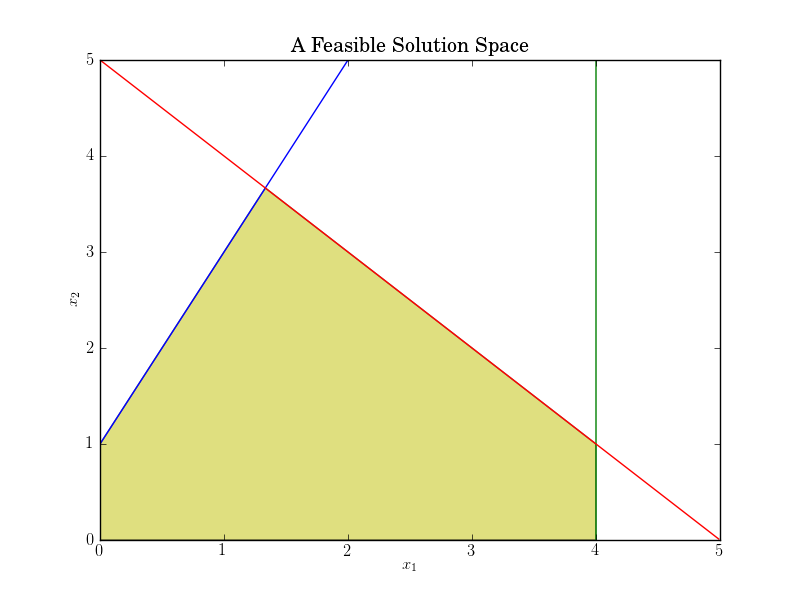
\includegraphics[width=\linewidth]{./chapters/litreview/plots/feasible.png}
  \caption{An example of a feasible solution space.}
  \label{fig:feasible}
  \end{center}
\end{figure}

The program can become infeasible by adjusting a constraint. Take for instance,
an increased boundary constraint for $x_2$.

%%% 
\begin{subequations}\label{eqs:infeas}
  \begin{align}
    %%
    \max \:\: & 
    3 x_1 + 2 x_2
    & \label{eqs:infeas_obj} \\
    %%
    \text{s.t.} \:\: &
    -2 x_1 + x_2 \leq 1 \\
    %%
    &
    x_1 + x_2 \leq 5 
    & \label{eqs:infeas_sup} \\
    %%
    &
    x_1 \in [0, 4]
    &\label{eqs:infeas_x1} \\
    %%
    &
    x_2 \geq 5
    &\label{eqs:infeas_x2}
    %%
  \end{align}
\end{subequations}
%%% 

This arrangement results in the infeasible linear program shown in
Figure \ref{fig:infeasible}, where the updated constraint's effect is shown in
red.

\begin{figure}[H]
  \begin{center}
    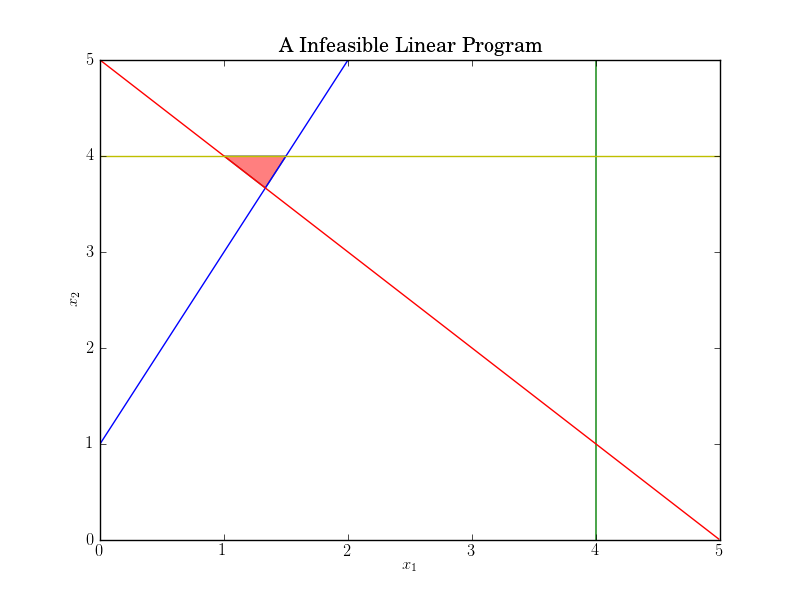
\includegraphics[width=\linewidth]{./chapters/litreview/plots/infeasible.png}
  \caption{An example of a infeasible solution space.}
  \label{fig:infeasible}
  \end{center}
\end{figure}

The standard form of a linear program shown in Equation \ref{eqs:std-form} is an
example of a \textit{primal} linear program. A distinction is made between
a \textit{primal} linear program and its \text{dual}. Duality theory is involved
and only treated lightly in this review. The standard form of the dual of
Equation \ref{eqs:std-form} is given in Equation \ref{eqs:dual-form}.

%%% 
\begin{subequations}\label{eqs:dual-form}
  \begin{align}
    %%
    \max_{u} \:\: & 
    w = b^{\top} u
    & \label{eqs:dual-form_obj} \\
    %%
    \text{s.t.} \:\: &
    A^{\top} u \leq c 
    & \label{eqs:dual-form_sup} \\
    %%
    &
    u \geq 0
    &\label{eqs:dual-form_x}
    %%
  \end{align}
\end{subequations}
%%% 

A few critical differences exist. First note that the objective directions are
switched: if a primal form has a minimization objective, its dual has a
maximization objective. The constraint matrix is now $M$ x $N$-dimensional (it
is in fact the original constraint matrix transposed). There is a new series of
decision variables that form the corresponding solution space, i.e., the
positive vector $u$, as shown in Equation \ref{eqs:dual-form_obj}. These
variables are related to the original right-hand side of the constraint
formulation, the vector $b$. The costs of the original problem, $c$, now form
the right-hand side of the dual's constraint formulation,
Equation \ref{eqs:dual-form_sup}.

The concept of duality is critical in the field of mathematical programming
because it provides well-defined optimality characteristics of a given
program. These are achieved via the \textit{Strong Duality Theorem}
and \textit{Weak Duality Theorem}, shown below as stated
in \cite{ferris_linear_2008}.

\begin{thm}[Weak Duality Theorem]
If $x$ is primal feasible and $u$ is dual feasible, then the dual objective
function evaluated at $u$ is less than or equal to the primal objective function
at $x$.
\end{thm}

The Weak Duality Theorem provides inextricable linkage between a primal feasible
solution and dual feasible solution. If a dual feasible solution is found, it
provides a lower bound on the optimal solution. If a primal feasible solution is
found, it provides an upper bound on the optimal solution. Both of these
criteria, in tandem, help to greatly reduce the required search space during
optimization sweeps.

\begin{thm}[Strong Duality Theorem]
Exactly one of the following three alternatives hold:
\begin{enumerate}

  \item Both primal and dual problems are feasible and consequently both have
  optimal solutions with \textit{equal} extrema

  \item \textit{Exactly one} of the problems is infeasible and consequently the
  other problem has and unbounded objective function in the direction of
  optimization on its feasible region

  \item \textit{Both} primal and dual problems are infeasible

\end{enumerate}
\end{thm}

The Strong Duality Theorem provides the backbone for much of linear programming
theory and application. It states that not only do feasible solutions to the
primal and dual programs provide upper and lower bounds on optimal values, but
that, in fact, the optimal values are \textit{equal}. This provides a criterion
to \textit{know} when an optimal value is reached.

With this slight overview of the realm of linear programming, one can move on to
solution techniques for problems that can be represented as linear programs.
